\section{Fonctionnement des Protocoles Wi-Fi}
\label{sec:protocoles}

La sécurité des réseaux Wi-Fi repose sur une succession de mécanismes cryptographiques introduits progressivement pour corriger les vulnérabilités de leurs prédécesseurs. Depuis \acrshort{wep} en 1997 jusqu'à \acrshort{wpa3} en 2018, chaque protocole a apporté des évolutions majeures : nouveaux algorithmes, nouvelles principes cryptographiques, mécanismes d'intégrité plus robustes, protection des trames de gestion, et résistance aux attaques hors ligne. Cette section propose une analyse approfondie de ces mécanismes, de leur logique interne, de leurs limites, ainsi que des structures de trames qu'ils manipulent.

\subsection{Principe général du Wi-Fi}

Le Wi-Fi, ou norme IEEE 802.11, désigne un ensemble de standards pour les réseaux locaux sans fil (WLAN) permettant la transmission de données numériques par ondes radio (principalement 2,4 GHz, 5 GHz et 6 GHz). Développé à partir des années 1990 par le comité IEEE 802.11 pour répondre à la demande croissante de connectivité mobile sans câblage Ethernet, le premier standard a été publié en 1997, révolutionnant l'accès aux données en éliminant les contraintes physiques des réseaux filaires.

Aujourd'hui, le Wi-Fi est omniprésent : hotspots publics (cafés, aéroports, transports), entreprises, foyers. Avec Wi-Fi 7 (802.11be, 2024) et au-delà, il supporte des débits >46 Gbit/s.

\subsection*{Définitions générales Wi-Fi}

Avant d’aborder en détail le fonctionnement des différents protocoles de sécurité, il est utile de préciser brièvement certains termes fondamentaux du Wi-Fi. Le \textbf{\acrfull{ssid}} correspond au nom d’un réseau et permet aux dispositifs de l’identifier lors de la phase de découverte. Le \textbf{\acrfull{bssid}}, quant à lui, désigne l’adresse MAC unique du point d’accès assurant la diffusion du réseau. Le terme \textbf{\acrfull{ap}} désigne ce même point d’accès, tandis que la \textbf{\acrfull{sta}} représente tout client Wi-Fi, qu’il s’agisse d’un ordinateur, d’un smartphone ou d’un objet connecté.

\begin{figure}[H]
\centering
\begin{tikzpicture}[>=latex, node distance=3cm]

% AP au centre
\node[draw, rounded corners, align=center, inner sep=4pt] (ap) {\acrfull{ap}\\[2pt]
\textbf{SSID} : \texttt{LabWiFi}\\
\textbf{BSSID} : \texttt{00:11:22:33:44:55}};

% Stations autour
\node[draw, rounded corners, left=of ap, align=center, inner sep=4pt] (sta1) {Station 1 (\acrshort{sta})\\PC portable};
\node[draw, rounded corners, right=of ap, align=center, inner sep=4pt] (sta2) {Station 2 (\acrshort{sta})\\Smartphone};
\node[draw, rounded corners, below=of ap, align=center, inner sep=4pt] (sta3) {Station 3 (\acrshort{sta})\\IoT / Objet connecté};

% Liens
\draw[<->] (ap) -- node[above]{Trames} (sta1);
\draw[<->] (ap) -- node[above]{Trames} (sta2);
\draw[<->] (ap) -- node[right]{Trames} (sta3);

\end{tikzpicture}
\caption{Illustration des notions \acrshort{ap}, \acrshort{sta}, \acrshort{ssid} et \acrshort{bssid} dans un réseau Wi-Fi}
\label{fig:ap_sta_ssid_bssid}
\end{figure}

Les communications Wi-Fi reposent sur des \glspl{trame} qui circulent au niveau de la couche MAC du modèle 802.11. On distingue notamment les trames de \textit{gestion}, essentielles pour l’association, l’authentification ou la déconnexion ; les trames de \textit{contrôle}, destinées à réguler l’accès au médium ; et les trames de \textit{données}, qui transportent l’information utilisateur ou les paquets réseau encapsulés. La plupart des attaques Wi-Fi tirent parti de la possibilité d’observer, d’injecter ou de manipuler ces différentes catégories de trames.

Enfin, plusieurs notions cryptographiques apparaissent régulièrement dans ce chapitre. La \textbf{\acrfull{pmk}} constitue le secret partagé à partir duquel toutes les clés de session sont dérivées, tandis que la \textbf{\acrfull{ptk}} correspond à la clé spécifique à la connexion entre un client et un point d’accès. La \textbf{\acrfull{gtk}} est utilisée pour chiffrer le trafic multicast ou broadcast adressé à plusieurs stations. Ces clés sont produites ou échangées dans le cadre de mécanismes tel que le 4-Way \Gls{handshake}, qui sera détaillé dans les sections suivantes.

Ces notions constituent le socle indispensable à la compréhension des protocoles de sécurisation Wi-Fi et des vulnérabilités qu’ils cherchent à prévenir.

\subsection*{Modes de mise en réseau \cite{WiFiWik42:online}}

Le Wi-Fi supporte plusieurs modes de mise en réseau, adaptés à des usages variés.

\paragraph{Mode Infrastructure}

Ce mode connecte les stations (\acrshort{sta}) via un ou plusieurs points d'accès (\acrshort{ap}) qui agissent comme des \glspl{concentrateur}. Initialement utilisé en entreprise pour poser des bornes à intervalles réguliers, il nécessite un \acrshort{ssid} commun pour la communication. L'avantage principal est le contrôle centralisé des accès : passage obligatoire par l'\acrshort{ap}. Aujourd'hui, les routeurs fournis par les \acrshort{fai} aux particuliers fonctionnent en mode infrastructure, faciles à configurer.

\begin{figure}[H]
\centering
\begin{tikzpicture}[
    box/.style={draw, rounded corners, minimum width=1.8cm, minimum height=0.8cm, align=center}
]
\node[box] (ap) {AP\\Routeur};
\node[box, left=2cm of ap] (sta1) {STA 1\\PC};
\node[box, right=2cm of ap] (sta2) {STA 2\\Phone};
\node[box, below=1.5cm of ap] (sta3) {STA 3\\IoT};
\draw[->] (ap) -- (sta1);
\draw[->] (ap) -- (sta2);
\draw[->] (ap) -- (sta3);
\node[font=\small, above=0.2cm of ap] {Mode Infrastructure};
\end{tikzpicture}
\caption{Mode Infrastructure : STA $\rightarrow$ AP central $\rightarrow$ Internet}
\end{figure}

\paragraph{Mode Ad hoc}

Ce mode permet une connexion directe entre stations sans point d'accès intermédiaire. Idéal pour des échanges rapides (fichiers entre portables dans un train ou un café), il repose sur un \acrshort{ssid}, un canal et une clé de chiffrement communs. Des protocoles de routage dynamique étendent la portée en mode maillé, où chaque nœud route pour les autres.

\begin{figure}[H]
\centering
\begin{tikzpicture}[
    box/.style={draw, rounded corners, minimum width=1.8cm, minimum height=0.8cm, align=center}
]
\node[box] (sta1) {STA 1\\PC};
\node[box, right=3cm of sta1] (sta2) {STA 2\\Phone};
\node[box, above right=1.5cm and 1cm of sta2] (sta3) {STA 3\\Laptop};
\draw[<->, thick] (sta1) -- (sta2);
\draw[<->, thick] (sta2) -- (sta3);
\draw[<->, dashed] (sta1) -- (sta3);
\node[font=\small, below=0.2cm of sta2] {Mode Ad hoc : Direct STA $\leftrightarrow$ STA};
\end{tikzpicture}
\caption{Mode Ad hoc : communication directe sans AP}
\end{figure}

\paragraph{Mode Pont (Bridge)}

Un \acrshort{ap} en mode pont relie d'autres \acrshort{ap} pour étendre un réseau filaire (ex. : entre bâtiments) au niveau couche 2 OSI. Un \acrshort{ap} racine distribue l'accès Internet, les autres se connectent en mode bridge et peuvent accueillir des clients comme en infrastructure.

\begin{figure}[H]
\centering
\begin{tikzpicture}[
    box/.style={draw, rounded corners, minimum width=1.8cm, minimum height=0.8cm, align=center}
]
\node[box] (root) {AP Racine\\Internet};
\node[box, right=3cm of root] (bridge1) {AP Bridge 1};
\node[box, right=3cm of bridge1] (bridge2) {AP Bridge 2};
\node[box, below=1cm of bridge2] (sta1) {STA 1};
\draw[<->, thick] (root) -- (bridge1);
\draw[<->, thick] (bridge1) -- (bridge2);
\draw[<->] (bridge2) -- (sta1);
\end{tikzpicture}
\caption{Mode Pont : extension réseau filaire via APs}
\end{figure}

\paragraph{Mode Répéteur (Range-extender)}

Ce mode étend la couverture en répétant le signal (ex. : fond de couloir). L'interface Ethernet reste inactive, mais chaque saut augmente la latence et divise le débit par deux (réception + retransmission sur la même antenne).

\begin{figure}[H]
\centering
\begin{tikzpicture}[
    box/.style={draw, rounded corners, minimum width=1.8cm, minimum height=0.8cm, align=center}
]
\node[box] (router) {Routeur\\principal};
\node[box, right=4cm of router] (repeater) {Répéteur};
\node[box, right=4cm of repeater] (sta) {STA\\Client};
\draw[<->] (router) -- node[midway, above] {Signal Wi-Fi 1} (repeater);
\draw[<->] (repeater) -- node[midway, above] {Signal Wi-Fi 2} (sta);
\end{tikzpicture}
\caption{Mode Répéteur : extension portée (débit /2, +latence)}
\end{figure}

\begin{table}[H]
\centering
\small
\begin{tabular}{|l|l|c|c|}
\hline
\textbf{Mode} & \textbf{Lien principal} & \textbf{Ethernet} & \textbf{Usage} \\
\hline
Infrastructure & STA $\rightarrow$ AP & \cmark & Internet \\
Ad hoc & STA $\leftrightarrow$ STA & \xmark & Échange direct \\
Pont & AP $\leftrightarrow$ AP (câble) & \cmark & Relier bâtiments \\
Répéteur & WiFi répété & \xmark & Étendre portée \\
\hline
\end{tabular}
\caption{Modes Wi-Fi : synthèse}
\label{tab:modes_wifi}
\end{table}

Ces modes fondamentaux conditionnent les mécanismes de sécurité analysés dans la suite, particulièrement en mode infrastructure dominant.


% WEP


\subsection{Sécurité Wi-Fi}

\subsubsection{WEP : Wired Equivalent Privacy}

\acrshort{wep} (1997) constitue la première tentative de sécuriser les communications Wi-Fi. Il a été conçu à une époque où la cryptographie grand public était encore émergente, et souffre aujourd'hui de nombreuses limitations. Son objectif était de fournir une confidentialité comparable à celle d'un réseau filaire, mais son fonctionnement s'est révélée profondément vulnérable.

\subsubsection*{Fonctionnement interne}

WEP repose sur l'algorithme de chiffrement par flot \acrshort{rc4}. Le mécanisme de chiffrement est simple :

\begin{itemize}
    \item une clé secrète partagée statique, nommée SharedKey (40 ou 104 bits) ;
    \item un \acrfull{iv} de 24 bits, envoyé en clair ;
    \item concaténation \texttt{IV || clé} comme entrée de RC4 ;
    \item un \acrfull{icv} calculé via CRC-32, ajouté au plaintext (\textit{texte en clair}) avant chiffrement.
\end{itemize}

Le chiffrement d'un paquet se fait ainsi :

\begin{figure}[H]
\centering
\begin{tikzpicture}[node distance=2cm]
\node[draw, rounded corners, inner sep=3pt] (in) {Input};
\node[draw, rounded corners, right=of in, inner sep=3pt] (pt) {Plaintext + ICV};
\node[draw, rounded corners, right=of pt, inner sep=3pt] (xor) {XOR};
\node[draw, rounded corners, below=of xor, inner sep=3pt] (rc4) {RC4};
\node[draw, rounded corners, left=of rc4, inner sep=3pt] (sk) {IV + SharedKey};
\node[draw, rounded corners, right=of rc4, inner sep=3pt] (ct) {IV + Ciphertext};
\node[draw, rounded corners, right=of ct, inner sep=3pt] (out) {Output};

\draw[->] (in) -- (pt);
\draw[->] (pt) -- (xor);
\draw[->] (rc4) -- (xor);
\draw[->] (xor) -- (ct);
\draw[->] (sk) -- (rc4);
\draw[->] (ct) -- (out);

\end{tikzpicture}
\caption{Principe du chiffrement WEP}
\label{fig:wep}
\end{figure}

\subsubsection*{Format d'une trame WEP}

\begin{figure}[H]
\centering
\begin{tikzpicture}[>=latex, node distance=0cm]

\node[
    draw,
    minimum width=3.2cm,
    minimum height=1.1cm,
    align=center
] (hdr) {802.11\\En-tête};

\node[
    draw,
    minimum width=2.2cm,
    minimum height=1.1cm,
    align=center,
    right=0.1cm of hdr
] (iv) {IV\\(24 bits)};

\node[
    draw,
    minimum width=4.8cm,
    minimum height=1.1cm,
    align=center,
    right=0.1cm of iv
] (data) {Données\\chiffrées (RC4)};

\node[
    draw,
    minimum width=2.5cm,
    minimum height=1.1cm,
    align=center,
    right=0.1cm of data
] (icv) {ICV\\(CRC-32)};

\end{tikzpicture}
\caption{Format d'une trame WEP}
\label{fig:wep-frame}
\end{figure}

\paragraph{Faiblesses cryptographiques majeures}

Le protocole WEP présente des faiblesses structurelles fondamentales :

\begin{itemize}
    \item \textbf{IV de 24 bits (16\,777\,216 valeurs possibles)} : chaque \gls{trame} WEP transmet son vecteur d'initialisation en clair. Avec un trafic normal, les collisions d'IV surviennent en quelques minutes (souvent moins de 5 minutes pour un \acrshort{ap} actif). Un attaquant peut alors combiner deux trames avec le même IV+clé pour annuler le keystream par XOR.
    
    \item \textbf{Aucun renouvellement de clé} : la clé secrète reste statique pendant des semaines/mois. Un \acrshort{iv} réutilisé expose la même clé \acrshort{rc4} pendant toute la durée de vie de la clé, permettant une attaque par collecte massive de trames.

    \item \textbf{ICV trop faible} : L’ICV s'appuie sur un algorithme peu robuste, il est possible de modifier des trames chiffrées sans connaître la clé, en recalculant un ICV valide.
\end{itemize}

\vspace{0.3cm}

Pour mieux comprendre le problème majeur de la taille de l'IV, nous allons prendre comme exemple : un IV est utilisé 2 fois $IV_0$, et deux messages combinés (données | \acrshort{icv}) $M_1$ et $M_2$.

\begin{enumerate}
    \item $IV_0$ $\rightarrow$ $RC4(IV_0||SharedKey) \oplus M_1 = C_1$
    \item $IV_0$ $\rightarrow$ $RC4(IV_0||SharedKey) \oplus M_2 = C_2$
    \item $C_1 \oplus C_2 = M_1 \oplus M_2$
    \item En-têtes IP (IP/TCP standardardisé) connus de $M_1$ $\rightarrow$ $M_2$ instantané
\end{enumerate}

En pratique, avec Aircrack NG, William Arbaugh note qu'il existe 50 \% de risque de collision après 4 823 paquets. \cite{Aircrack74:online}
La documentation conseille elle 250,000 IVs pour des clés de 64 bit et 1,500,000 IVs pour des clés de 128 bit. \cite{simplewe40:online}

\newpage


% WPA

\subsubsection{WPA : Wi-Fi Protected Access}

Face à la crise WEP, la Wi-Fi Alliance introduit en 2003 \acrshort{wpa} comme correctif transitoire, visant à remplacer les composants vulnérables tout en conservant le matériel existant (compatibilité ascendante).
WPA s'appuie sur un problème de chiffrement nommé \acrfull{tkip}.

\subsubsection*{Fonctionnement interne}

WPA introduit plusieurs mécanismes :
\begin{itemize}
    \item un mélange de clés élaboré (phase 1 et phase 2) ;
    \item un \acrlong{iv} de taille doublée (24 à 48 bits) ; 
    \item un \acrfull{tsc} pour de l'anti-replay ;
    \item un \acrfull{mic} pour de l'intégrité et de la signature ;
    \item une rotation des clés fréquente.
\end{itemize}

\subsubsection*{Phases de WPA}

Le protocole s'appuie sur une clé connue par les \acrshort{sta} et l\acrshort{ap}, nommée \acrfull{psk}. Il peut également, dans le cadre de \textit{WPA-Enterprise}, être généré via un serveur RADIUS.
Ici, nous ne développerons que la méthode avec une passphrase connue par les deux parties.

WPA corrige WEP par 3 étapes distinctes :

\begin{itemize}
    \item \textbf{Phase 1 (\acrshort{pbkdf2} 4096 itérations)} : passphrase $\rightarrow$ \acrfull{pmk} résistante plus robuste. Cette clé n'est jamais utilisée directement, elle ne sert qu'à générer une clé temporaire.\\La fonction PBKDF2 utilise le SSID comme sel cryptographique et applique 4096 itérations de HMAC-SHA1. Ce mécanisme ralentit volontairement les tentatives de brute force, mais n'empêche pas les attaques hors ligne si la passphrase est faible et que le 4-Way Handshake est capturé.


    \begin{figure}[H]
        \centering
        % Schéma 1 : Phase 1
        \begin{tikzpicture}[
            box/.style={draw, rounded corners, minimum width=2cm, minimum height=0.9cm, align=center}
        ]
        \node[box] (psk) {\acrlong{psk}\\passphrase};
        \node[box, right=1.8cm of psk] (pbkdf2) {PBKDF2\\Dérivation de clé};
        \node[box, right=1.8cm of pbkdf2] (pmk) {Pairwise Master Key\\(256 bits)};

        \draw[->] (psk) -- (pbkdf2);
        \draw[->] (pbkdf2) -- (pmk);
        \end{tikzpicture}
        \caption{Phase 1 : Sécurisation de la clé}
        \label{fig:wpa_phase_1}
    \end{figure}

    
    \item \textbf{Phase 2 (4-Way \Gls{handshake})} : \acrshort{pmk} $\rightarrow$ \acrshort{ptk} échangée sans jamais transmettre la clé (\Gls{anonce}/\Gls{snonce} + \acrshort{mic} protègent).
    \\Les nonces (\Gls{anonce} et \Gls{snonce}) garantissent l'unicité de la PTK à chaque association, même si la PMK reste identique. Le \acrshort{mic}, calculé à l'aide de la clé KCK, assure l'intégrité et l'authenticité des messages du handshake.

    
    \begin{figure}[H]
        \centering
        % Schéma 2 : Phase 2  
        \begin{tikzpicture}[
            box/.style={draw, rounded corners, minimum width=2cm, minimum height=0.9cm, align=center}
        ]
        \node[box] (pmk2) {PMK};
        \node[box, right=1.8cm of pmk2] (handshake) {4-Way Handshake};
        \node[box, right=1.8cm of handshake] (ptk) {Pairwise Transient Key\\512 bits};

        \draw[->] (pmk2) -- (handshake);
        \draw[->] (handshake) -- (ptk);
        \end{tikzpicture}
        \caption{Phase 2 : Création d'une clé unique en \acrshort{ap} et \acrshort{sta}}
        \label{fig:wpa_phase_2}
    \end{figure}

    % 4-Way Handshake
    Le \textbf{4-Way Handshake} assure 3 objectifs critiques :

    \begin{itemize}
        \item \textbf{Preuve mutuelle PMK} : \acrshort{sta} et \acrshort{ap} prouvent qu'ils connaissent la même PMK sans jamais la transmettre.
        
        \item \textbf{PTK (Pairwise Transient Key, 512 bits)} : clé unique unicast \acrshort{sta} $\leftrightarrow$ \acrshort{ap}, dérivée de : 
        \[
            \begin{aligned}
            PTK = PRF(&PMK, \\
                    &\min(MAC_{AP}, MAC_{STA}) \, || \, \max(MAC_{AP}, MAC_{STA}) \, || \\
                    &\min(\Gls{anonce}, \Gls{snonce}) \, || \, \max(\Gls{anonce}, \Gls{snonce})
            )
            \end{aligned}
        \].
        
        \item \textbf{GTK (Group Temporal Key)} : clé broadcast/multicast partagée par TOUS les clients du réseau (trafic groupe). L'\acrshort{ap} l'envoie chiffrée avec la PTK du client.
    \end{itemize}

    \begin{figure}[H]
    \centering
    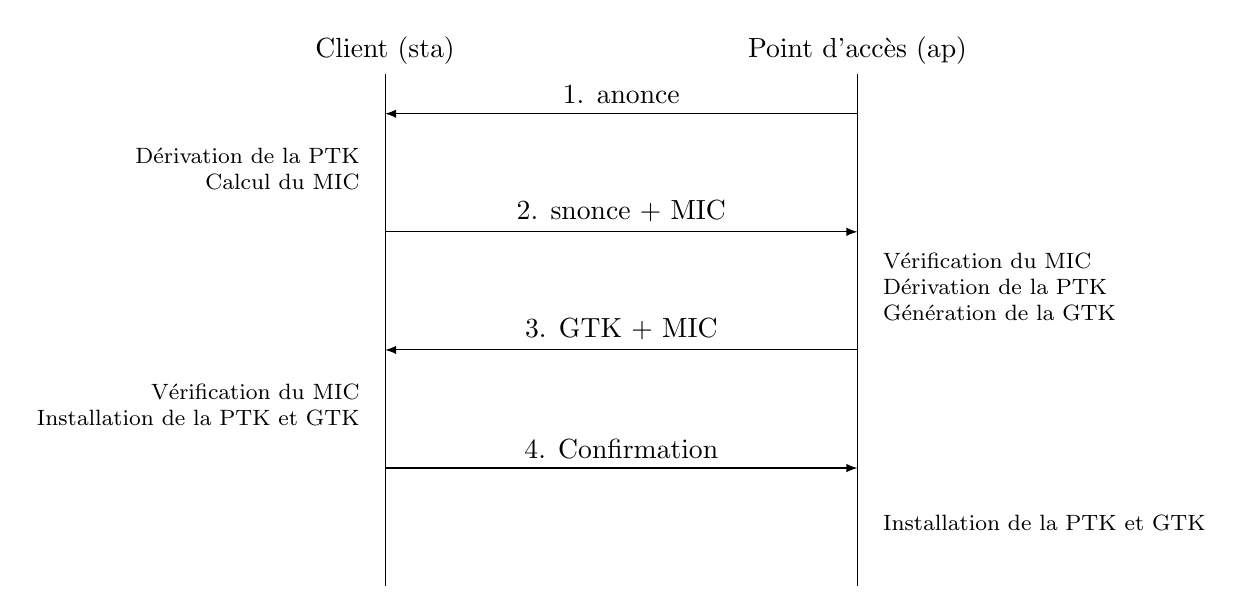
\begin{tikzpicture}[>=latex]

    \node (sta) at (0,0) {Client (\acrshort{sta})};
    \node (ap)  at (6,0) {Point d'accès (\acrshort{ap})};

    % Lignes de vie
    \draw (sta.south) -- ++(0,-6.5);
    \draw (ap.south)  -- ++(0,-6.5);

    % Messages
    \draw[->] (ap.south)++(0,-0.5) -- node[above,sloped]{1. \Gls{anonce}} ++(-6,0);
    \draw[->] (sta.south)++(0,-2) -- node[above,sloped]{2. \Gls{snonce} + MIC} ++(6,0);
    \draw[->] (ap.south)++(0,-3.5) -- node[above,sloped]{3. GTK + MIC} ++(-6,0);
    \draw[->] (sta.south)++(0,-5) -- node[above,sloped]{4. Confirmation} ++(6,0);

    % Étapes locales STA (à gauche)
    \node[anchor=east, align=right, font=\footnotesize] 
    at (-0.2,-1.5) {%
    Dérivation de la PTK\\
    Calcul du MIC
    };

    \node[anchor=east, align=right, font=\footnotesize] 
    at (-0.2,-4.5) {%
    Vérification du MIC\\
    Installation de la PTK et GTK
    };

    % Étapes locales AP (à droite)
    \node[anchor=west, align=left, font=\footnotesize] 
    at (6.2,-3) {%
    Vérification du MIC\\
    Dérivation de la PTK\\
    Génération de la GTK
    };

    \node[anchor=west, align=left, font=\footnotesize] 
    at (6.2,-6.0) {%
    Installation de la PTK et GTK
    };

    \end{tikzpicture}
    \caption{4-Way Handshake WPA/WPA2}
    \label{fig:4way}
    \end{figure}

    La \textit{Pairwise Transient Key} (PTK) est en pratique un trousseau de sous-clés spécialisées : la KCK est utilisée pour l’authentification et la protection des messages du 4-Way Handshake, la KEK pour chiffrer et distribuer la clé de groupe GTK, et la TK pour chiffrer le trafic de données unicast entre la STA et le point d’accès.

    \begin{figure}[H]
        \centering
        \begin{tikzpicture}[
            box/.style={draw, rounded corners, minimum width=2.4cm, minimum height=0.9cm, align=center},
            smallbox/.style={draw, rounded corners, minimum width=2.2cm, minimum height=0.8cm, align=center, font=\footnotesize}
        ]

        \node[box] (ptk) {PTK\\(512 bits)};

        \node[smallbox, below=1.2cm of ptk] (kek) {\acrfull{kek}\\128 bits};
        \node[smallbox, left=0.2cm of kek] (kck) {\acrfull{kck}\\128 bits};
        \node[smallbox, right=0.2cm of kek] (tk) {\acrlong{tk}\\256 bits};

        \draw[->] (ptk) -- (kck);
        \draw[->] (ptk) -- (kek);
        \draw[->] (ptk) -- (tk);
        \end{tikzpicture}
        \caption{Décomposition de la PTK en sous-clés KCK, KEK et TK.}
        \label{fig:ptk-subkeys}
    \end{figure}

    \begin{table}[H]
        \centering
        \begin{tabular}{|l|l|l|l|l|l|}
        \hline
        \textbf{Clé} &
        \textbf{Taille} &
        \textbf{Usage} &
        \textbf{Phase} &
        \textbf{Renouvellement} \\
        \hline
        PSK &
        Variable &
        Passphrase partagée &
        Pré-Phase &
        Manuel \\

        PMK &
        256 bits &
        Clé maître dérivée (PBKDF2) &
        Phase 1 &
        À chaque authentification \\

        PTK &
        512 bits &
        Clé transitoire unicast &
        Phase 2 &
        À chaque 4-Way Handshake \\

        KCK &
        128 bits &
        Intégrité du handshake (MIC) &
        Phase 2 &
        À chaque 4-Way Handshake \\

        KEK &
        128 bits &
        Chiffrement de la GTK &
        Phase 2 &
        À chaque 4-Way Handshake \\

        TK &
        256 bits &
        Chiffrement des données unicast &
        Phase 3 & Clé par paquet (via TSC) \\

        GTK &
        128 bits &
        Trafic broadcast/multicast &
        Phase 2 &
        Périodique / Reconnexion \\
        \hline
        \end{tabular}
        \caption{Récapitulatif des clés utilisées dans WPA-TKIP}
        \label{tab:wpa_keys}
    \end{table}

    \item \textbf{Phase 3 (TKIP par trame)} : une fois les clés installées, chaque trame de données est chiffrée indépendamment à l'aide de TKIP. 
        Contrairement à WEP, une clé unique est générée pour chaque paquet.

        Pour chaque trame, les éléments suivants sont utilisés :
        \begin{itemize}
            \item la clé temporaire TK ;
            \item l'adresse MAC de l'émetteur ;
            \item le \acrfull{tsc} (compteur anti-rejeu de 48 bits).
        \end{itemize}

        TKIP applique un \textbf{mélange de clés en deux phases} :
        \begin{itemize}
            \item \textbf{Phase 1} : combine la TK, la MAC source et les 32 bits de poids fort du TSC pour produire une clé intermédiaire ;
            \item \textbf{Phase 2} : intègre les 16 bits de poids faible du TSC afin de générer la clé RC4 finale spécifique au paquet.
        \end{itemize}

        Un \acrshort{mic} (Michael) est ensuite calculé sur les données en clair avant chiffrement, 
        puis l'ensemble est chiffré à l'aide de RC4 et transmis.

    \begin{figure}[H]
        \centering
        \begin{tikzpicture}[
            box/.style={draw, rounded corners, minimum width=2.6cm, minimum height=0.9cm, align=center}
        ]
        \node[box] (data) {Données claires};
        \node[box, below=0.8cm of data] (mic) {Calcul MIC};
        \node[box, below=0.8cm of mic] (mix) {Key Mixing TKIP};
        \node[box, below=0.8cm of mix] (rc4) {Chiffrement RC4};
        \node[box, below=0.8cm of rc4] (frame) {Trame Wi-Fi chiffrée};

        \draw[->] (data) -- (mic);
        \draw[->] (mic) -- (mix);
        \draw[->] (mix) -- (rc4);
        \draw[->] (rc4) -- (frame);
        \end{tikzpicture}
        \caption{Chiffrement d'une trame WPA-TKIP}
        \label{fig:wpa_tkip_frame}
        \end{figure}
\end{itemize}

Bien que RC4 soit toujours utilisé, WPA réduit significativement les risques d'attaque sans néanmoins les éliminer.

% WPA2

\subsubsection{WPA2 : AES-CCMP et le 4-Way Handshake}

WPA2 apporte une amélioration profonde : l’abandon de RC4 au profit d’un chiffrement moderne AES-CCMP.

\subsubsection*{Modes d’authentification}
\begin{itemize}
    \item \textbf{WPA2-PSK} : la PMK (\textit{Pairwise Master Key} : clé maitresse) = PBKDF2(\textit{Password-Based Key Derivation Function 2} : basée sur une passphrase et le SSID).
    \item \textbf{WPA2-Enterprise} : PMK fournie via un serveur RADIUS et une authentification EAP.
\end{itemize}


% PMK -> PTK -> GTK derivation

\subsubsection{Dérivation des clés}

Au-delà de l’échange de messages représenté dans la Figure~\ref{fig:4way}, le 4-Way Handshake repose sur un mécanisme de dérivation de clés particulièrement structuré. L’ensemble du processus débute avec la PMK (Pairwise Master Key), qui constitue la base cryptographique partagée entre le client et le point d’accès. Dans le cas d’un réseau WPA2-PSK, cette PMK résulte directement de l’application d’une fonction de dérivation (PBKDF2) sur la passphrase et le SSID ; dans un environnement Enterprise, elle est fournie après l’authentification EAP par un serveur RADIUS. L’objectif du handshake n’est donc pas de négocier une nouvelle clé, mais de prouver que les deux entités possèdent bien cette PMK sans jamais la transmettre.

À partir de cette PMK, les deux parties vont dériver une clé plus large appelée PTK (Pairwise Transient Key). La construction de la PTK repose sur plusieurs éléments : l’adresse MAC du point d’accès, celle du client, ainsi que deux valeurs aléatoires appelées \Gls{anonce} (envoyée par l’AP) et SNonce (envoyée par la station). Ces quatre paramètres garantissent que la PTK générée est unique pour chaque session, même si la PMK reste identique : une propriété essentielle pour éviter la réutilisation de clés et limiter les risques d’attaque par rejeu ou par corrélation.

La PTK n’est pas utilisée directement ; elle est découpée en trois sous-clés distinctes, chacune remplissant un rôle spécifique dans la sécurisation du lien. La première est la KCK (Key Confirmation Key), employée pour calculer les MIC (Message Integrity Code) des messages du handshake. Elle permet à chaque partie de vérifier que l’autre possède bien la PTK correcte, et donc implicitement la PMK. La deuxième sous-clé est la KEK (Key Encryption Key), utilisée par l’AP pour chiffrer la GTK (Group Temporal Key) transmise dans le message~3. Cette clé assure que seul un client légitime peut recevoir ou mettre à jour la clé de diffusion. Enfin, la dernière composante est la TK (Temporal Key), qui servira au chiffrement effectif du trafic unicast échangé entre la station et l’AP après la fin du handshake.

Un autre élément important est la présence de la GTK, envoyée par le point d’accès lors du message~3 du 4-Way Handshake. Contrairement à la PTK, qui est propre à une paire client–AP, la GTK est partagée entre tous les clients d’un même réseau et sert au chiffrement des trames multicast et broadcast. Sa transmission protégée par la KEK garantit qu’un attaquant passif ne peut pas l’intercepter, tandis que son renouvellement régulier limite les risques de compromission en cas d’écoute prolongée.

Ainsi, le 4-Way Handshake ne se réduit pas à un simple échange de valeurs nonces, mais constitue un véritable protocole d’initialisation cryptographique. Il assure simultanément la preuve de possession du secret initial, la dérivation de clés fraîches, l’établissement d’un canal chiffré sécurisé et la synchronisation des compteurs de trames. L’ensemble du mécanisme repose sur des propriétés formelles destinées à garantir la confidentialité et l’intégrité des échanges, tout en minimisant les risques liés à la réutilisation ou à la dérivation incorrecte des clés.

\begin{figure}[H]
\centering
\begin{tikzpicture}[>=latex, node distance=1.8cm]

\node[draw, rounded corners, inner sep=4pt] (pmk) {PMK};
\node[draw, rounded corners, below=of pmk, inner sep=4pt] (prf) {PRF(PMK, nonces, MAC)};
\node[draw, rounded corners, below=of prf, inner sep=4pt] (ptk) {PTK = KCK || KEK || TK};
\node[draw, rounded corners, right=3cm of ptk, inner sep=4pt] (gtk) {GTK};

\draw[->] (pmk) -- (prf);
\draw[->] (prf) -- node[left]{4-way handshake} (ptk);
\draw[->] (ptk.east) -- node[above]{KEK} (gtk.west);

\end{tikzpicture}
\caption{Dérivation cryptographique PMK $\rightarrow$ PTK $\rightarrow$ GTK}
\end{figure}


% CCMP frame format

\subsubsection*{Format d'une trame CCMP (WPA2)}

\begin{figure}[H]
\centering
\begin{tikzpicture}
\node[draw, minimum width=3cm] (hdr) {802.11 Header};
\node[draw, minimum width=2cm, right=0cm of hdr] (pn) {PN};
\node[draw, minimum width=2cm, right=0cm of pn] (ccmp) {CCMP Header};
\node[draw, minimum width=4cm, right=0cm of ccmp] (data) {Payload (AES-CTR)};
\node[draw, minimum width=3cm, right=0cm of data] (mic) {MIC (CBC-MAC)};
\end{tikzpicture}
\caption{Structure d'une trame CCMP}
\end{figure}


% WPA3 / SAE

\subsubsection{WPA3 : SAE, Dragonfly, GCMP et PMF}

WPA3 corrige des failles structurelles de WPA2, notamment KRACK, en introduisant SAE (Dragonfly), OWE, PMF obligatoire, et le support obligatoire de GCMP dans certaines suites.

\subsubsection*{Handshake SAE (Dragonfly)}

\begin{figure}[H]
\centering
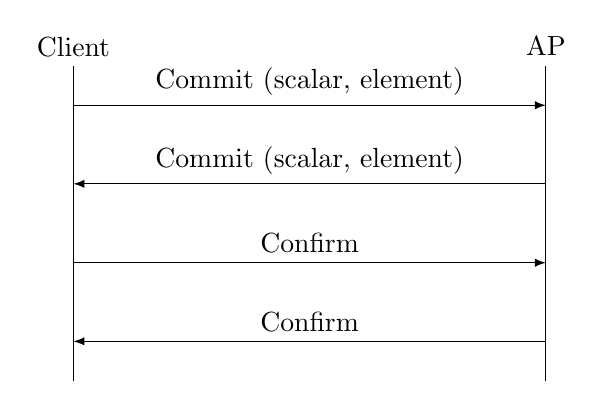
\begin{tikzpicture}[>=latex]

\node (sta) at (0,0) {Client};
\node (ap)  at (6,0) {AP};

\draw (sta.south) -- ++(0,-4);
\draw (ap.south)  -- ++(0,-4);

\draw[->] (sta.south)++(0,-0.5) -- node[above,sloped]{Commit (scalar, element)} ++(6,0);
\draw[->] (ap.south)++(0,-1.5) -- node[above,sloped]{Commit (scalar, element)} ++(-6,0);
\draw[->] (sta.south)++(0,-2.5) -- node[above,sloped]{Confirm} ++(6,0);
\draw[->] (ap.south)++(0,-3.5) -- node[above,sloped]{Confirm} ++(-6,0);

\end{tikzpicture}
\caption{Handshake SAE (WPA3)}
\end{figure}


% SAE / GCMP crypto details

\subsection{Mécanismes cryptographiques avancés}

Les protocoles de sécurité modernes du Wi-Fi reposent sur des mécanismes cryptographiques plus élaborés que ceux utilisés par les générations précédentes. Contrairement à WEP et TKIP, qui n’offraient qu’une protection minimale contre l’écoute, l’injection ou la manipulation des trames, WPA2 et surtout WPA3 reposent sur des constructions cryptographiques complètes, conçues pour fournir à la fois confidentialité, intégrité, résistance aux attaques par rejeu et garanties formelles sur la sécurité de la session. Trois mécanismes occupent une place centrale : AES-CCMP, GCMP et SAE (aussi appelé Dragonfly). Ces primitives ne jouent pas le même rôle, mais constituent ensemble la base de la sécurité Wi-Fi contemporaine.

\subsubsection{AES-CCMP}

AES-CCMP est devenu la norme de chiffrement par défaut avec WPA2. Son objectif est d’aller bien au-delà du simple masquage des données transportées : il assure simultanément la confidentialité des informations, l’intégrité des trames et la protection contre les attaques par rejeu.

Pour y parvenir, CCMP combine deux éléments complémentaires. D’une part, il utilise AES en mode compteur (CTR) pour le chiffrement. Ce mode transforme le bloc AES en générateur de flot chiffrant, permettant de chiffrer efficacement des paquets de taille variable sans introduire de structure exploitable. De l’autre, CCMP associe ce chiffrement à un code d’authentification basé sur CBC-MAC, un mécanisme cryptographique destiné à garantir que les données n’ont subi aucune altération. Cette combinaison forme une construction dite \textit{AEAD} (Authenticated Encryption with Associated Data), dans laquelle confidentialité et intégrité sont assurées simultanément par une même clé, ce qui évite un grand nombre de vulnérabilités présentes dans les générations antérieures.

L’ensemble repose également sur un numéro de paquet (Packet Number, PN) utilisé comme nonce unique. Toute réutilisation est interdite, ce qui empêche un attaquant de rejouer ou de réinjecter des trames chiffrées. En pratique, AES-CCMP constitue encore aujourd’hui une référence en matière de chiffrement pour les réseaux Wi-Fi.

AES-CCMP combine :
\begin{itemize}
    \item AES en mode CTR pour le chiffrement ;
    \item CBC-MAC pour l'intégrité (authentification).
\end{itemize}
C'est une construction AEAD robuste, largement testée.

\subsubsection{GCMP (AES-GCM)}

GCMP, introduit avec les standards 802.11ac et repris dans WPA3-Enterprise, reprend les principes d’AES-CCMP mais s’appuie cette fois sur AES-GCM. Cette construction fait partie des modes de chiffrement AEAD les plus étudiés et les plus robustes. AES-GCM associe un chiffrement en mode CTR à la fonction d’authentification GHASH, reposant sur des opérations arithmétiques dans un corps de Galois. Cette approche permet de calculer l’intégrité et le chiffrement de façon quasi parallèle, ce qui rend GCMP particulièrement performant sur les architectures modernes.

L’intérêt principal de GCMP réside donc dans sa rapidité : il offre un débit supérieur à CCMP, ce qui le rend bien adapté aux environnements à forte charge ou aux réseaux professionnels nécessitant des débits élevés. Il reste néanmoins sensible aux erreurs d’implémentation, comme l’ont montré certaines variantes des attaques Dragonblood qui ciblaient directement GCMP-128 lorsque les nonces n’étaient pas utilisés correctement. Malgré cela, GCMP demeure une brique cryptographique robuste lorsqu’il est correctement mis en œuvre.

\subsubsection{SAE / Dragonfly}


Contrairement à AES-CCMP et à GCMP, qui sont des mécanismes de chiffrement et d’intégrité utilisés \emph{après} l’établissement de la connexion, SAE (Simultaneous Authentication of Equals) intervient au moment de l’authentification. SAE n’est pas un algorithme de chiffrement mais un protocole d’échange de clés sécurisé, faisant partie de la famille des PAKE (Password-Authenticated Key Exchange).

L’enjeu de SAE est de résoudre l’un des problèmes fondamentaux des versions antérieures : avec WPA2-PSK, un attaquant pouvait capturer un 4-Way Handshake puis tenter hors ligne de retrouver le mot de passe par dictionnaire. Dans SAE, ce type d’attaque est impossible. Le protocole s'appuie sur un échange Diffie–Hellman (sur groupes modp ou courbes elliptiques), dans lequel le mot de passe n'est jamais transmis ni dérivé sous forme exploitable. Chaque tentative d’authentification nécessite une interaction en temps réel avec le point d’accès, ce qui empêche les attaques hors ligne et limite naturellement la vitesse des tests possibles.

SAE offre également la propriété de \textit{Forward Secrecy} : même si un mot de passe venait à être compromis ultérieurement, les sessions passées resteraient inexploitables, car la clé de session résulte d’un secret éphémère renouvelé à chaque connexion. Cette approche corrige l’une des failles conceptuelles les plus importantes de WPA2 et constitue la principale amélioration de WPA3-Personal.

Pour résumer, ses caractériques principales sont les suivantes :

\begin{itemize}
    \item s’appuie sur Diffie-Hellman (modp ou ECC) ;
    \item offre Forward Secrecy ;
    \item empêche les attaques hors-ligne ;
    \item protège contre attaques dictionnaires massives.
\end{itemize}


% Format de trame GCMP

\subsubsection*{Format d'une trame GCMP}

\begin{figure}[H]
\centering
\begin{tikzpicture}
\node[draw, minimum width=3cm] (hdr) {802.11 Header};
\node[draw, minimum width=2cm, right=0cm of hdr] (pn) {PN};
\node[draw, minimum width=2cm, right=0cm of pn] (gcmp) {GCMP Header};
\node[draw, minimum width=4cm, right=0cm of gcmp] (data) {Payload (AES-GCM)};
\node[draw, minimum width=3cm, right=0cm of data] (tag) {Tag (128 bits)};
\end{tikzpicture}
\caption{Structure d'une trame GCMP (WPA3)}
\end{figure}


% Synthesis table

\subsection{Synthèse comparative approfondie}

\begin{table}[H]
\centering
\begin{tabular}{|c|c|c|c|c|}
\hline
\textbf{Protocole} & \textbf{Crypto} & \textbf{Auth} & \textbf{Intégrité} & \textbf{Résistance} \\
\hline
WEP & RC4 & Clé statique & CRC-32 & Nulle \\
WPA & RC4 & PSK & MIC & Faible \\
WPA2 & AES-CCMP & PSK/802.1X & CBC-MAC & Forte (hors KRACK) \\
WPA3 & AES-CCMP/GCMP & SAE/802.1X & PMF & Très forte \\
OWE & Diffie-Hellman & Aucune & CCMP/GCMP & Élevée \\
\hline
\end{tabular}
\caption{Comparaison des protocoles de sécurité Wi-Fi}
\end{table}

\newpage